\documentclass[12pt, a4paper, onecolumn]{IEEEtran}
% https://www.monash.edu/rlo/quick-study-guides/writing-a-case-study
\usepackage{url} % for typesetting URLs
\usepackage{hyperref}
\usepackage{cleveref}
\hypersetup{
	colorlinks=true,
	linkcolor=blue,
	filecolor=blue,
	citecolor=blue,
	urlcolor=magenta,
}
\usepackage[style=ieee]{biblatex}

% Citation Needed Command
\usepackage{xcolor}
\newcommand{\citationneeded}{[\textcolor{blue}{citation needed}]}

\usepackage{caption}
\usepackage{subcaption}
\usepackage{graphicx}
\graphicspath{ {./pictures/} }

%% Bibliography
\addbibresource{./bibliography.bib}

\title{An Overview of Chordophone Actuation}
\author{Joshua Benfell}

\begin{document}

	\maketitle
    \section{Introduction}
        Humans are mechanically fluid and complex with the ability to produce a wide range of minute differences for similar motions. 
        As such, many methods of picking a stringed instrument are present, from picking individual strings to strumming. 
        Methods further vary in expressiveness due to properties such as the angle of attack and volume.
        Such a wide range of possibilities is reflected in the variation of existing mechanisms.
        Furthermore, damping strings, to prevent certain tones, is an integral part of playing instruments due to the dynamics introduced.
    \section{Picking Mechanisms}

        \begin{figure}[!h]
            \centering
            \begin{subfigure}{0.3\textwidth}
                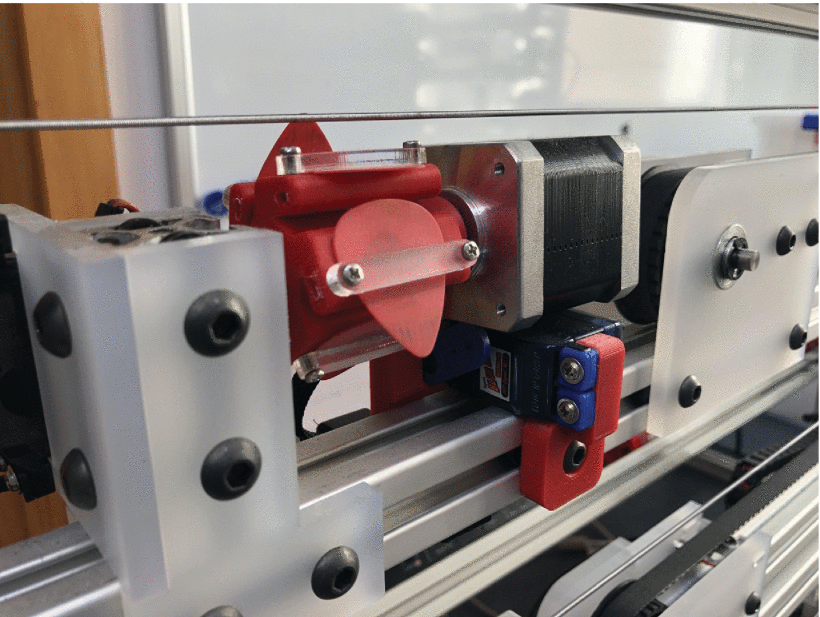
\includegraphics[width=\columnwidth]{mechbass_picking.png}
                \subcaption{Mechbass Picking Mechanism \cite{VUW_Chordophones}}
                \label{fig:mechbass_picking}
            \end{subfigure}
            \begin{subfigure}{0.2\textwidth}
                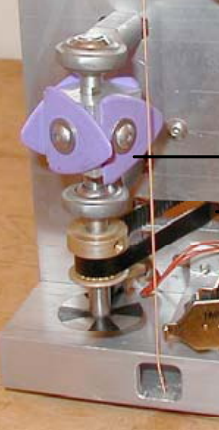
\includegraphics[width=\columnwidth]{guitarbot_picking.png}
                \subcaption{GuitarBot Picking Mechanism \cite{GuitarBot}}
                \label{fig:guitarbot_picking}
            \end{subfigure}
            \caption{Rotary Picking Mechanisms}
            \label{fig:RotaryPicking}
        \end{figure}

        
        Mechanisms for picking individual strings commonly consist of a drum that rotates multiple plectra, as seen with Mechbass \cite{VUW_Chordophones}, GuitarBot \cite{GuitarBot}, or the use of a solenoid to actuate plectra over a string \cite{PWM_Solenoid,Silent_Picking,Pivot_Picking}. 
        Rotary mechanisms make use of a drum of equally spaced plectra that rotate to strike the string.
        Solenoid based picking methods, work by using one or two solenoids to push and pull a plectra over a string.
        % As is evident in \Cref{fig:SolenoidPicking}, these are generally considerably larger than the rotary variant.
        
        \begin{figure}[!h]
            \centering
            \begin{subfigure}{0.2\textwidth}
                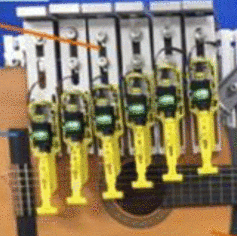
\includegraphics[width=\columnwidth]{silent_picking.png}
                \subcaption{\cite{Silent_Picking}}
                \label{fig:silent_picking}
            \end{subfigure}
            \begin{subfigure}{0.3\textwidth}
                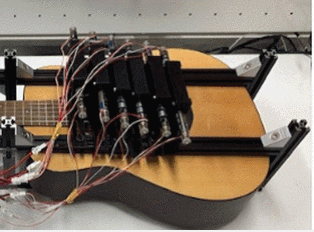
\includegraphics[width=\columnwidth]{pwmSolenoid_picking.png}
                \subcaption{\cite{PWM_Solenoid}}
                \label{fig:pwm_picking}
            \end{subfigure}
            \begin{subfigure}{0.3\textwidth}
                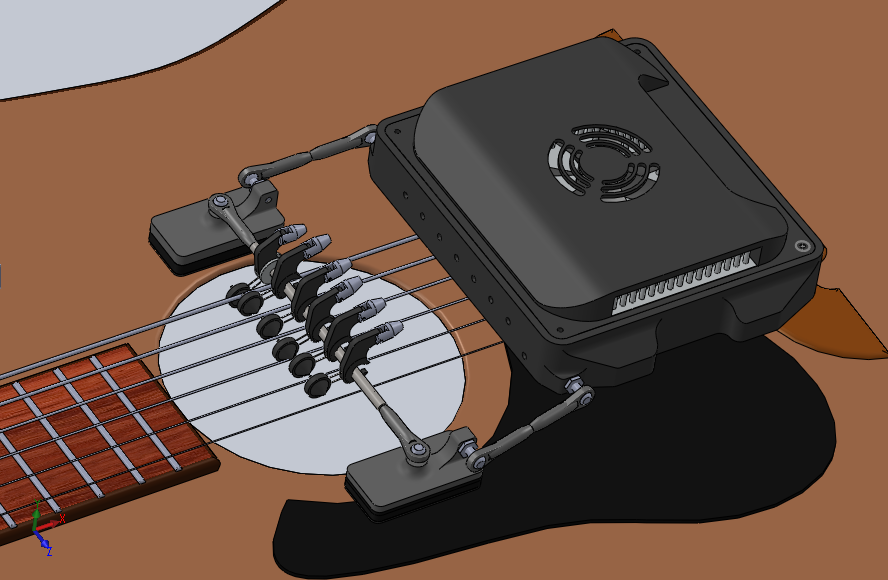
\includegraphics[width=\columnwidth]{pivotSolenoid_picking.png}
                \subcaption{\cite{Pivot_Picking}}
                \label{fig:pivot_picking}
            \end{subfigure}
            \caption{Solenoid Based Picking Mechanisms}
            \label{fig:SolenoidPicking}
        \end{figure}

        These picking mechanism are both capable of speeds greater than what is reasonably acheivable by humans \cite{pickspeed}. 
        Rotary designs offer greater flexibility as increasing the drum size increases the maximum picking speed through an increase in pick count and speed \cite{VUW_Chordophones,pickspeed}.
        In contrast, solenoids have fixed speeds, making an increase require a different actuator, with slower speeds capable through the use of PWM control \cite{PWM_Solenoid}.
        However, rotary methods require aligning multiple plectra so that the sound is consistent through a full rotation.

        When it comes to physical size, solenoid mechanisms are considerably larger than rotary counterparts as they are typically designed across the string \cite{VUW_Chordophones,Silent_Picking,PWM_Solenoid}.
        However, by making the pick a small rubber cone, the size of the actuator is reduce while keeping some compliance \cite{Pivot_Picking}.
        As this design was capable of fitting on the guitar adjacently, it is possible, that a solenoid actuator is applicable to monochord setups.
        However, the ability to vary the pick attack is sacrificed.

        Due to the ability to vary the speed at which the plectra crosses the string, the two groups of actuation are capable of varying the volume of the sound produced, with higher speeds resulting in higher volumes \cite{PWM_Solenoid}.
        However, what they lack is the ability to change how the pick crosses the string.
        Mechbass utilises a servo to move the picker, altering where the plectra strikes the string, with closer causing increased volume \cite{VUW_Chordophones}. 
        Further expressiveness can be added by changing the attack angle. 
        % Neither of these adjustments have been attempted with solenoids, however, this is due to the rotary system being simpler to move and adjust due to the size and layout.

        Actuating strings introduces many noise sources, both electromagnetic and mechanial, which effects the result.
        Both motor types can be picked up by magnetic pickups, so it is important to place these well to reduce this without introducing weaknesses or altering the sound significantly, however, optical sensors have proved successful if more complex \cite{VUW_Chordophones}.
        Further, to reduce mechanical noise from solenoids, an elastic membrance can be used to lower impact and reduce sound to 2dB above background noise \cite{Silent_Picking}.

        
    \section{Damping Mechanisms}
        \begin{figure}[!h]
            \centering
            \begin{subfigure}{0.35\textwidth}
                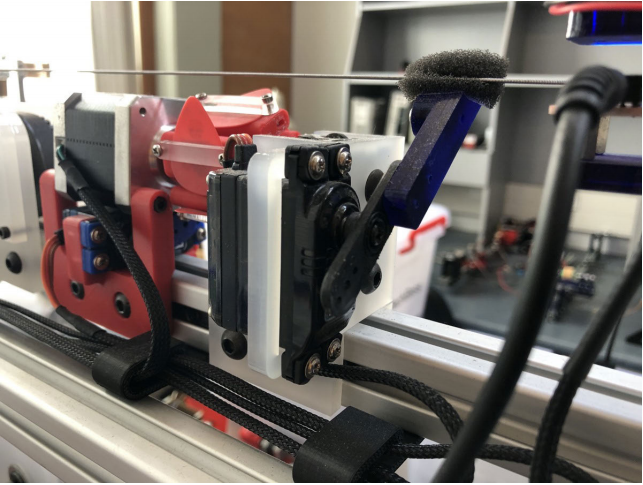
\includegraphics[width=\columnwidth]{mechbass_damping.png}
                \subcaption{Foam Servo Damping Mechanism\cite{VUW_Chordophones}}
                \label{fig:mechbass_damping}
            \end{subfigure}
            \begin{subfigure}{0.4\textwidth}
                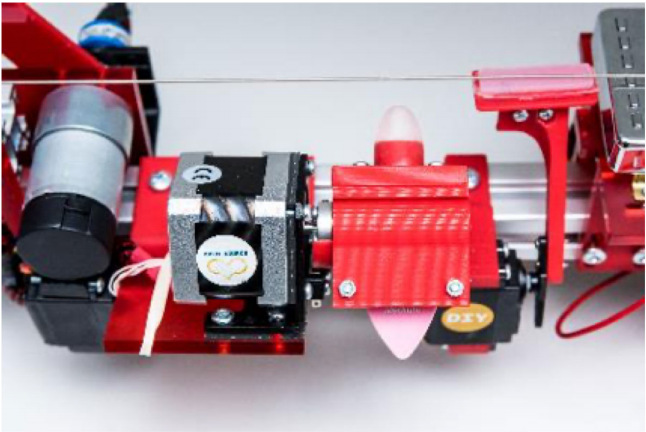
\includegraphics[width=\columnwidth]{silicone_damping.png}
                \subcaption{Silicone Servo Damping Mechanism\cite{VUW_Chordophones}}
                \label{fig:pwm_picking}
            \end{subfigure}
            \caption{Damping Mechanisms}
            \label{fig:silicone_damping}
        \end{figure}


        Damping mechanisms generally consist of a servo with foam, felt or silicone making contact with the string, with silicone being the most like human skin \cite{VUW_Chordophones}.
        They have been used at points near the picking mechanism, and the pitch shifter, as these create different results \cite{VUW_Chordophones}.
        Typically these have been used to fully mute strings, however, it is possible to partially mute, with lighter touches.
        Where these mechanisms fall short is in controlled decay of the sound, as they have only been used to move to set positions.
        Further development for damping mechanisms would be to explore playing actively with the damping through slap muting.


    \section{Conclusion}
        When it comes to picking, it is apparent that rotary mechanisms offer more flexibility and control as you are able to easy modify them through the drum, and can provide them with an accurate velocity and position them precisely. 
        They are smaller than solenoid systems, allowing addition to the systems pick attack and more dynamics.
        There is a lack of detail about stepper motor noise in the literature, so solenoids seem the quieter option using a bespoke spring.
        Further research areas to focus on for picking would be the development of an actuator that is capable of varying attack angle and distance, particularly without introducing too much electromagnetic noise, as reducing the need for a precision optical sensor improves accessibility.

        Damping systems are reasonably based for simple implementations, however, they are lacking in the control of the damping with feedback as identified by \cite{VUW_Chordophones}.
        Additionally, there is little literature on picking with a muted string, or slapping the string while playing.

    \printbibliography

\end{document}